\section{Generalized Minimum Residual Method (GMRES)}
Let $\mathcal{K} = \mathcal{K}_m(A, \mathbf{r}_0)$, and $\mathcal{L}_m = A\mathcal{K}$.
\begin{align*}
    \mathbf{r}_m                     & = \mathbf{b} - A\mathbf{x}_m                                                                                                                                                                    \\
    \|\mathbf{b} - A\mathbf{x}_m\|_2 & = \min_{\mathbf{x} \in \mathbf{x}_0 + \mathcal{K}_m} \|\mathbf{b} - A\mathbf{x}\|_2                                                                                                             \\
    \mathbf{x}                       & \in \mathbf{x}_0 + \mathcal{K}_m \quad \Rightarrow \quad \mathbf{x} = \mathbf{x}_0 + V_m \mathbf{y}_m, \quad \mathbf{y}_m \in \mathbb{R}^m                                                      \\
    \mathbf{r}                       & = \mathbf{b} - A\mathbf{x} = \mathbf{b} - A(\mathbf{x}_0 + V_m \mathbf{y}_m) = \mathbf{r}_0 - AV_m \mathbf{y}_m                                                                                 \\
                                     & = \mathbf{r}_0 - V_{m+1} \overline{H}_m \mathbf{y}_m                                                                                                                                            \\
                                     & = V_{m+1}(\beta \mathbf{e}_1 - \overline{H}_m \mathbf{y}_m)                                                                                                                                     \\
    \|\mathbf{r}\|^2                 & = \|V_{m+1}(\beta \mathbf{e}_1 - \overline{H}_m \mathbf{y}_m)\|_2 = \|\beta \mathbf{e}_1 - \overline{H}_m \mathbf{y}_m\|_2, \quad \text{since } \|V_{m+1}\|_2 = 1 \text{ (orthonormal columns)} \\
    \mathbf{y}_m                     & = \arg\min_{\mathbf{y} \in \mathbb{R}^m} \|\beta \mathbf{e}_1 - \overline{H}_m \mathbf{y}\|_2                                                                                                   \\
    \mathbf{x}_m                     & = \mathbf{x}_0 + V_m \mathbf{y}_m
\end{align*}
Want to solve the overdetermined system ($m < n$):
\[
    \overline{H}_m \mathbf{y} \approx \beta \mathbf{e}_1
\]
We solve this least squares problem using QR factorization of $\overline{H}_m$ with Givens rotations.

\subsection{QR Factorization Approach}
Since $\overline{H}_m \in \mathbb{R}^{(m+1) \times m}$ is upper Hessenberg, we can efficiently compute its QR factorization using Givens rotations. Let
\[
    \overline{H}_m = Q_{m+1} R_m
\]
where $Q_{m+1} \in \mathbb{R}^{(m+1) \times (m+1)}$ is orthogonal and $R_m \in \mathbb{R}^{(m+1) \times m}$ has the structure:
\[
    \tilde{R}_m = \begin{bmatrix}
        R_m \\
        \mathbf{0}^\top
    \end{bmatrix}
\]
with $R_m \in \mathbb{R}^{m \times m}$ upper triangular.

Let
\[
    \bar\mathbf{g}_m = Q_{m+1}^\top \beta \mathbf{e}_1 = [\gamma_1, \gamma_2, \ldots, \gamma_{m+1}]^\top
\]

The least squares problem becomes:
\begin{align*}
    Q_m\left(\beta \mathbf{e}_1 - \overline{H}_m \mathbf{y}\right) & = \beta Q_m \mathbf{e}_1 - Q_m \overline{H}_m \mathbf{y}
    = \overbrace{\beta Q_m \mathbf{e}_1}^{\bar{\mathbf{g}}_m}- \begin{bmatrix}R_m \\ \mathbf{0}^\top \end{bmatrix} \mathbf{y}_m                                                                     \\
                                                                   & = \begin{bmatrix} \mathbf{g}_{1:m} \\g_{m+1} \end{bmatrix} - \begin{bmatrix} R_m \\ \mathbf{0}^\top \end{bmatrix} \mathbf{y}_m \\
                                                                   & = \begin{bmatrix}\mathbf{g}_{1:m} - R_m \mathbf{y}_m \\ g_{m+1} \end{bmatrix}
\end{align*}

Then:
\begin{align*}
    \|\beta \mathbf{e}_1 - \overline{H}_m \mathbf{y}\|^2 & = \|\bar\mathbf{g}_m - \tilde{R}_m \mathbf{y}\|^2 = \|\mathbf{g}_{1:m} - R_m \mathbf{y}\|^2 + |g_{m+1}|^2 \\
    \mathbf{y}_m                                         & = R_m^{-1} \mathbf{g}_{1:m}                                                                               \\
    \|\mathbf{r}_m\|_2                                   & = |\gamma_{m+1}|
\end{align*}
Then we do QR factorization by Givens rotations:
\begin{align*}
    h                             & = \begin{bmatrix}
                                          h_1 \\
                                          h_2
                                      \end{bmatrix}, \quad
    \Omega = \begin{bmatrix}
                 c  & s \\
                 -s & c
             \end{bmatrix}, \quad c^2 + s^2 = 1                                                              \\
    \Omega h                      & = \begin{bmatrix}
                                          \|h\| \\
                                          0
                                      \end{bmatrix}                                                         \\
    \begin{bmatrix}
        c  & s \\
        -s & c
    \end{bmatrix} \begin{bmatrix}
                      h_1 \\
                      h_2
                  \end{bmatrix} & = \begin{bmatrix}
                                        r \\
                                        0
                                    \end{bmatrix}                                                           \\
    \Rightarrow \quad \|h\|       & = \sqrt{h_1^2 + h_2^2}, \quad c = \frac{h_1}{r}, \quad s = \frac{h_2}{r}
\end{align*}
In the Arnoldi process for $k=1$:
\begin{align*}
    H_1                & = \begin{bmatrix}
                               h_{1,1} \\
                               h_{2,1}
                           \end{bmatrix} \xrightarrow{\Omega_1} \begin{bmatrix}
                                                                    \tilde{h}_{1,1} \\
                                                                    0
                                                                \end{bmatrix} \\
    \beta \mathbf{e}_1 & = \begin{bmatrix}
                               \beta \\
                               0
                           \end{bmatrix} \xrightarrow{\Omega_1} \begin{bmatrix}
                                                                    \gamma_1 \\
                                                                    \gamma_2
                                                                \end{bmatrix}
\end{align*}
For $k=2$:
\begin{align*}
    H_2             & = \begin{bmatrix}
                            \tilde{h}_{1,1} & h_{1,2} \\
                            0               & h_{2,2} \\
                            0               & h_{3,2}
                        \end{bmatrix} \xrightarrow{\Omega_2} \begin{bmatrix}
                                                                 \tilde{h}_{1,1} & \tilde{h}_{1,2} \\
                                                                 0               & \tilde{h}_{2,2} \\
                                                                 0               & 0
                                                             \end{bmatrix} \\
    \begin{bmatrix}
        \gamma_1 \\
        \gamma_2 \\
        \gamma_3
    \end{bmatrix} & \xrightarrow{\Omega_2} \begin{bmatrix}
                                               \gamma_1         \\
                                               \tilde{\gamma}_2 \\
                                               \tilde{\gamma}_3
                                           \end{bmatrix}
\end{align*}

after $m$ iterations we have:
\begin{align*}
    \tilde{R}_m      & = \begin{bmatrix}
                             \tilde{h}_{1,1} & \tilde{h}_{1,2} & \cdots & \tilde{h}_{1,m} \\
                             0               & \tilde{h}_{2,2} & \cdots & \tilde{h}_{2,m} \\
                             0               & 0               & \cdots & \tilde{h}_{3,m} \\
                             \vdots          & \vdots          & \ddots & \vdots          \\
                             0               & 0               & \cdots & 0
                         \end{bmatrix} \\
    \bar\mathbf{g}_m & = \begin{bmatrix}
                             \gamma_1 \\
                             \gamma_2 \\
                             \vdots   \\
                             \gamma_{m+1}
                         \end{bmatrix}
    =
    \begin{bmatrix}
        g_{1:m} \\
        g_{m+1}
    \end{bmatrix}
\end{align*}

Afer $k$ iterates:
\begin{align*}
    \begin{bmatrix}
        h_{1,k} \\
        h_{2,k} \\
        \vdots  \\
        h_{k,k} \\
        h_{k+1,k}
    \end{bmatrix}
     & \xrightarrow{\Omega_k}
    \begin{bmatrix}
        \gamma_1 \\
        \gamma_2 \\
        \vdots   \\
        \gamma_k \\
        0
    \end{bmatrix}
\end{align*}
before applying Givens rotations.
\[
    \|r_{k-1}\| = |\gamma_k|
\]
Then Givens:
\begin{align*}
    \begin{bmatrix}
        c_k  & s_k \\
        -s_k & c_k
    \end{bmatrix}
    \begin{bmatrix}
        \gamma_k \\
        0
    \end{bmatrix}
            & =
    \begin{bmatrix}
        c_k \gamma_k \\
        -s_k \gamma_k
    \end{bmatrix}                                  \\
    \|r_k\| & = |-s_k \gamma_k| = |s_k| \|r_{k-1}\|
\end{align*}

Then
\begin{align*}
    |s_k|            & \leq 1                                                                                                               \\
    \text{If } |s_k| & < 1, \text{ then } \|r_k\| < \|r_{k-1}\|                                                                             \\
    \text{If } |s_k| & = 1, \text{ then stagnation, but then } c_k = 0 \text{ which means } h_{k, k} = 0 \text{ or } A \text{ is singular.} \\
    c_k              & = \frac{h_{k,k}}{\sqrt{h_{k,k}^2 + h_{k+1,k}^2}}, \qquad s_k = \frac{h_{k+1,k}}{\sqrt{h_{k,k}^2 + h_{k+1,k}^2}}
\end{align*}

\subsubsection{GMRES Algorithm}
\begin{algorithm}[H]
    \caption{GMRES Algorithm}
    \begin{algorithmic}
        \State $\mathbf{r}_0 = \mathbf{b} - A\mathbf{x}_0$
        \State $\beta = \|\mathbf{r}_0\|_2$
        \State $\mathbf{v}_1 = \frac{\mathbf{r}_0}{\beta}$
        \For{$j = 1, 2, \ldots, m$}
        \State $\mathbf{w}_j = A\mathbf{v}_j$
        \For{$i = 1, 2, \ldots, j$}
        \State $h_{ij} = \langle \mathbf{w}_j, \mathbf{v}_i \rangle$
        \State $\mathbf{w}_j = \mathbf{w}_j - h_{ij} \mathbf{v}_i$
        \EndFor
        \State $h_{j+1,j} = \|\mathbf{w}_j\|_2$
        \If{$h_{j+1,j} = 0$} \textbf{Stop}
        \EndIf
        \State $\mathbf{v}_{j+1} = \frac{\mathbf{w}_j}{h_{j+1,j}}$
        \EndFor
        \State $V_m = [\mathbf{v}_1, \mathbf{v}_2, \ldots, \mathbf{v}_m] \in \mathbb{R}^{n \times m}$
        \State $V_m^\top V_m = I$
        \State $H_m \in \mathbb{R}^{m \times m}$
        \State $\overline{H}_j \in \mathbb{R}^{(m+1) \times m}$ (upper Hessenberg matrix)
        \State Compute minimizer $\mathbf{y}_m$ of $\|\beta \mathbf{e}_1 - \overline{H}_m \mathbf{y}\|_2$
        \State $\mathbf{x}_m = \mathbf{x}_0 + V_m \mathbf{y}_m$ (Solution)
    \end{algorithmic}
\end{algorithm}

\subsection{Convergence of GMRES}
We want to estimate the convergence of GMRES. We have:
\begin{itemize}
    \item $\mathbf{x}_\star$ exact solution of $A\mathbf{x} = \mathbf{b}$.
    \item $\mathbf{x}_m$ numerical solution after $m$ iterations with some \emph{krylov-space method}.
          \begin{align*}
              \mathbf{r}_m &= \mathbf{b} - A\mathbf{x}_m \tag{residual error} \\
              \mathbf{x}_\star - \mathbf{x}_m & = p_m(A)(\mathbf{x}_\star - \mathbf{x}_0)
              \quad
              \begin{cases}
                p_m \in \mathbb{P}_m\\
                p_m(0) = 1
                \end{cases} \\
              \mathbf{b} - A\mathbf{x}_m      & = p_m(A)(\mathbf{b} - A\mathbf{x}_0)                                                  \\
              \mathbf{r}_m                    & = p_m(A)\mathbf{r}_0
          \end{align*}
\end{itemize}

Let $\mathcal{L}_m = A\mathcal{K}_m$.

\begin{align*}
    \|\mathbf{r}_m\|_2 & = \min_{\mathbf{x} \in \mathbf{x}_0 + \mathcal{K}_m} \|\mathbf{b} - A\mathbf{x}\|_2 \\
    \|\mathbf{r}_m\|_2 & \leq \|\mathbf{r}_{m-1}\|_2 \leq \ldots \leq \|\mathbf{r}_0\|_2
\end{align*}
For each $\|\mathbf{r}_0\|_2$ it is possible to find an $A$ s.t.
\[
    \|\mathbf{r}_m\|_2 = \|\mathbf{r}_{m-1}\|_2 = \ldots = \|\mathbf{r}_0\|_2
\]
Here $A$ may not be diagonalizable, but we assume it is, s.t.
\[
    A = X\Lambda X^{-1}
\]
but where $X$ is not orthogonal anymore.
\begin{align*}
    p(A)               & = Xp(\Lambda)X^{-1}                                                                                                                 \\
    \mathbf{r}_m       & = p_m(A)\mathbf{r}_0 = Xp_m(\Lambda)X^{-1}\mathbf{r}_0                                                                              \\
    \|\mathbf{r}_m\|_2 & \leq \|X\|_2 \|X^{-1}\|_2 \max_{1 \leq i \leq n} |p_m(\lambda_i)| \|\mathbf{r}_0\|_2                                                \\
                       & = \sqrt{\lambda_{\max}(A^H A) \cdot \lambda_{\min}((A^H A)^{-1})} \max_{1 \leq i \leq n} |p_m(\lambda_i)| \|\mathbf{r}_0\|_2        \\
                       & = \kappa_2(X) \max_{1 \leq i \leq n} |p_m(\lambda_i)| \|\mathbf{r}_0\|_2                                                            \\
    \kappa_2(X)        & = \|X\|_2 \|X^{-1}\|_2 = \sqrt{\lambda_{\max}(A^H A)\cdot \lambda_{\min}((A^H A)^{-1})} = \frac{\sigma_{\max}(X)}{\sigma_{\min}(X)}
\end{align*}
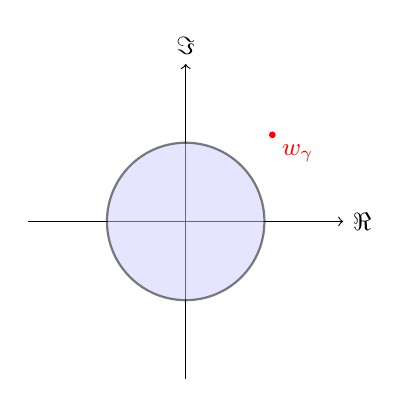
\begin{tikzpicture}[font=\small]
    % Im, Re axes
    \draw[->] (-2, 0) -- (2, 0) node[right] {$\Re$};
    \draw[->] (0, -2) -- (0, 2) node[above] {$\Im$};
    % circle
    \draw[thick, fill=blue!20, opacity=0.5] (0, 0) circle (1);
    % w_g just outside the circle
    \filldraw[red] (1.1, 1.1) circle (1pt) node[below right] {$w_\gamma$};
\end{tikzpicture}
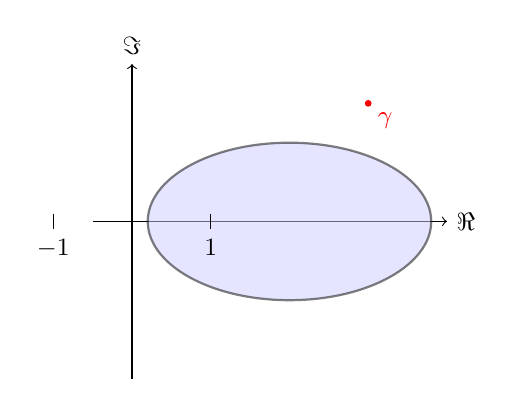
\begin{tikzpicture}[font=\small]
    % Im, Re axes
    \draw[->] (-0.5, 0) -- (4, 0) node[right] {$\Re$};
    \draw[->] (0, -2) -- (0, 2) node[above] {$\Im$};
    % Ellipse
    \draw[thick, fill=blue!20, opacity=0.5] (2, 0) ellipse (1.8 and 1);
    % -1, 1 ticks
    \draw (-1, 0.1) -- (-1, -0.1) node[below] {$-1$};
    \draw (1, 0.1) -- (1, -0.1) node[below] {$1$};
    % gamma just outside the ellipse
    \filldraw[red] (3, 1.5) circle (1pt) node[below right] {$\gamma$};
\end{tikzpicture}
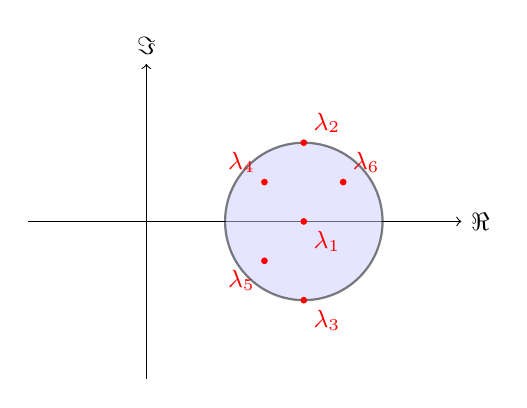
\begin{tikzpicture}[font=\small]
    % Im, Re axes
    \draw[->] (-1.5, 0) -- (4, 0) node[right] {$\Re$};
    \draw[->] (0, -2) -- (0, 2) node[above] {$\Im$};

    % Circle at (2,0) with radius 1
    \draw[thick, fill=blue!20, opacity=0.5] (2, 0) circle (1);

    % Eigenvalues
    \filldraw[red] (2, 0) circle (1pt) node[below right] {$\lambda_1$};
    \filldraw[red] (2, 1) circle (1pt) node[above right] {$\lambda_2$};
    \filldraw[red] (2, -1) circle (1pt) node[below right] {$\lambda_3$};
    \filldraw[red] (1.5, 0.5) circle (1pt) node[above left] {$\lambda_4$};
    \filldraw[red] (1.5, -0.5) circle (1pt) node[below left] {$\lambda_5$};
    \filldraw[red] (2.5, 0.5) circle (1pt) node[above right] {$\lambda_6$};
\end{tikzpicture}

Let $\lambda_i \in \mathrm{E}$ for $i = 1, \ldots, n$, where $\mathrm{E}$ is a closed ellipse, and $D_\rho := \{w \in \mathbb{C} : |w| = \rho\}$.
We search for some $p^\star$ solving the min-max problem:
\[
    \min_{\substack{p \in \mathbb{P}_m \\ p(0) = 1}} \max_{\lambda_i \in \mathrm{E}} |p(\lambda)|
\]

\subsubsection{Chebyshev polynomials in $\mathbb{C}$}

let $z \in \mathbb{C}$:
\begin{align*}
    C_m(z)     & = \cosh(m \cdot \rho), \quad \rho = \cosh^{-1}(z)                 \\
    w          & = e^{\rho}                                                        \\
    C_m(z)     & = \frac{1}{2}(e^{m\rho} + e^{-m\rho}) = \frac{1}{2}(w^m + w^{-m}) \\
    C_{m+1}(z) & = 2zC_m(z) - C_{m-1}(z), \quad C_0(z) = 1, \, C_1(z) = z          \\
    z          & = \frac{1}{2}(w + w^{-1})
\end{align*}

\begin{lemma}{Zarantonello}{}
    Let $\gamma \in \mathbb{C}$, $|\gamma| > \rho$, then:
    \[
        \min_{\substack{p \in \mathbb{P}_m \\ p(\gamma) = 1}} \max_{w \in D_\rho} = \left(\frac{\rho}{|\gamma|}\right)^m
    \]
    Minimal polynomial is given by:
    \[
        p(z) = \left(\frac{z}{\gamma}\right)^m
    \]
    Max is obtained when $z = \rho$.
\end{lemma}

\subsubsection{Joukowsky mapping}
\begin{align*}
    J(w)      & = \frac{1}{2}(w + w^{-1}), \quad w \in \mathbb{C}, \, w \neq 0 \\
    J(D_\rho) & = \mathrm{E}(0,1, \frac12(\rho + \rho^{-1}))
\end{align*}
\begin{theorem}{Elman}{}
    Let $J(D_\rho) = \mathrm{E}_\rho$ and choose $\gamma$ outside $\mathrm{E}_\rho$, and let  $ w_\gamma = J^{-1}(\gamma)$ (the biggest), then:
    \begin{align*}
        \frac{\rho^m}{|w_\gamma|^m} & \leq \min_{\substack{p \in \mathbb{P}_m \\ p(\gamma) = 1}} \max_{z \in \mathrm{E}_\rho} |p(z)| \leq \frac{\rho^m + \rho^{-m}}{|w_\gamma^m + w_\gamma^{-m}|}
    \end{align*}
    Then the optimal polynomial $p^\star$ is given by:
    \[
        p^\star(w) = \frac{w^m + w^{-m}}{w_\gamma^m + w_\gamma^{-m}}, \quad w \in \mathbb{C}
    \]
    is close to our optimal polynomial when $m$ is large.
\end{theorem}

\begin{align*}
    C_m(z)                                        & = \frac{1}{2}(w^m + w^{-m}), \quad z = \frac{1}{2}(w + w^{-1})                                                          \\
    p^\star(z)                                    & = \frac{C_m(w)}{C_m(w_\gamma)}                                                                                          \\
    \hat{C}_m(z)                                  & = \frac{C_m(\frac{z - c}{d})}{C_m(-\frac{c}{d})},
    \begin{cases}
        \mathrm{E}(c,d,a), \\
        \hat{C}_m(0) = 1
    \end{cases}                                                                                                                                   \\
    \max_{z \in \mathrm{E}(c,d,a)} |\hat{C}_m(z)| & = \frac{C_m(\frac{a}{d})}{|C_m(-\frac{c}{d})|}                                                                          \\
    \mathbf{r}_m                                  & \leq \kappa_2(X) \varepsilon^{m} \|\mathbf{r}_0\|_2 = \kappa_2(X) \frac{C_m(\frac{a}{d})}{|C_m(-\frac{c}{d})|} \|\mathbf{r}_0\|_2                                           \\
    C_m(z)                                        & = \frac{1}{2}\left[\left(z + \sqrt{z^2 - 1}\right)^m + \left(z - \sqrt{z^2 - 1}\right)^m\right]                         \\
    \varepsilon^m                                 & = \frac{C_m(\frac{a}{d})}{|C_m(-\frac{c}{d})|} \approx \left(\frac{a + \sqrt{a^2 - d^2}}{c + \sqrt{c^2 - d^2}}\right)^m
\end{align*}

The ellipse enclosing the eigenvalues can not include $0$, because then $p(0) = 1$ can not be satisfied.
If $a < c$, then we have convergene for sure.

